% !TEX root = ../probability_hse_exams.tex
\thispagestyle{empty}
\section{Решения контрольной номер 1. ИП}


\subsection[2023-2024, ип]{\hyperref[sec:kr_01_ip_2023_2024]{2023-2024, ип}}
\label{sec:sol_kr_01_ip_2023_2024}


\subsection[2023-2024, эад]{\hyperref[sec:kr_01_ead_2023_2024]{2023-2024, эад}}
\label{sec:sol_kr_01_ead_2023_2024}


\subsection[2022-2023]{\hyperref[sec:kr_01_ip_2022_2023]{2022-2023}}
\label{sec:sol_kr_01_ip_2022_2023}

\begin{enumerate}
  \item $p_a = \P(X \leq 3) = 1 - \exp(-3\lambda_N)$, 
  \begin{align*}
  F(1) = 1 - \P(X / (N+1)>1) = 1 - \sum_{k=0} \P(N = k) \P(X > k+1) = \\
  = 1 - \sum \exp(-\lambda_N) \frac{\lambda_N^k}{k!} \exp( - (k+1)\lambda_X) = \\
  = 1 - \exp(-\lambda_N - \lambda_X) \sum \frac{(\lambda_N \exp(-\lambda_X))^k}{k!} = \\
  = 1 - \exp(-\lambda_N - \lambda_X + \lambda_N \exp(-\lambda_X))
  \end{align*}
  \item 
  \item Вероятность того, что мячи попадут одному человеку равна $p = 1/(n-2)$. 
  Замечаем, что количество раундов распределено геометрически, это количество испытаний до первого успеха. 
  Отсюда $\E(X) = 1/p$ и $\P(X = 2) = (1-p) p$.
  \item $\P(X=1)=0.2$, $\P(X=2)=0.3$, $\P(X=3)=0.5$, $g'(1) = \E(X)$.
  \item $T = \min\{ X_1, X_2, X_3 \}$, $\E(T) = 5/4$.
\end{enumerate}


\subsection[2021-2022]{\hyperref[sec:kr_01_ip_2021_2022]{2021-2022}}
\label{sec:sol_kr_01_ip_2021_2022}

\begin{enumerate}
  \item x
  \item Исходное равенство 
\[
  \P(X \geq 1) + \cdots + \P(X \geq 10) = 5
\]
можно представить в виде
\[
  \P(X = 1) + 2 \P(X = 2) + \cdots + 10\P(X = 10) = \E(X) = 5
\]

Также можно заметить, что по смыслу исходное равенство — это площадь над функцией распределения 
для неотрицательной случайной величины. 
  \item x
  \item[4a.]
\begin{enumerate}
  \item Сначала найдём вероятности:
  \[
  \P(\lceil X \rceil = k) = F_X(k) - F_X(k-1) = \exp(-k+1) - \exp(-k), \text{ при } k \in \mathbb N.
  \]
  Можно переписать вероятности в виде:
  \[
    \P(\lceil X \rceil = k) = (\exp(-1))^{k-1}(1 - \exp(-1)).
  \]
  Вероятности соответствуют геометрическому распределению с вероятностью успеха $p = 1 - \exp(-1)$.
  Следовательно, $\E\lceil X \rceil = 1/ (1 - \exp(-1))$.

  \item Обозначим ошибку округления как $R = \lceil X \rceil - X$. 
  \[
  \P(R \in [r;r+dr]) = \P(X\in [1-r-dr; 1-r]) + \P(X\in [2-r-dr; 2-r]) + \ldots
  \]
  
  Рассмотрим отрезок малой длины $dr$, $\P(X\in [1-r-dr; 1-r]) = \P(X\in [1-r; 1-r+dr]) + o(dr)$.
  
  \[
  f_R(r) dr = f_X(1-r)dr + f_X(2-r)dr + \ldots = (\exp(r-1) + \exp(r-2) + \ldots) dr = \frac{\exp(r-1)}{1 - \exp(-1)}dr
  \]

  Домножаем на $\exp(1)$ и получаем 
  \[
  f_R(r) = \exp(r)/(\exp(r) - 1).  
  \]

\end{enumerate}
  \item[4b.] Обозначим количество дней до искоренения преступности буквой $D$. 
  Замечаем, что искомая функция $f(n, w) = \E(D)$ пропорциональна $n$. 
  Чтобы изловить всех преступников, надо сначала поймать первого и его последователей,
  потом второго и его последователей и так далее. 
  Методом первого шага получаем уравнение
  \[
  f(1, w) = 1 + 0.05 w f(1, w).  
  \]
  Отсюда 
  \[
  f(n, w) = \frac{n}{1-0.05w}.
  \]

  Альтернативное решение 4b.

  Замечаем, что за каждый день число преступников в среднем падает на $1 - 0.05w$. 
  Получаем 
  \[
  \E(D) = n / (1 - 0.05w).
  \]

  Оценивание: пункт а = 5 баллов, пункт б = 10 баллов.

\end{enumerate}


\subsection[2020-2021]{\hyperref[sec:kr_01_ip_2020_2021]{2020-2021}}
\label{sec:sol_kr_01_ip_2020_2021}



\subsection[2019-2020]{\hyperref[sec:kr_01_ip_2019_2020]{2019-2020}}
\label{sec:sol_kr_01_ip_2019_2020}

\begin{enumerate}
  \item xxx
  \item xxx
  \item 

  \begin{minipage}{0.3\textwidth}
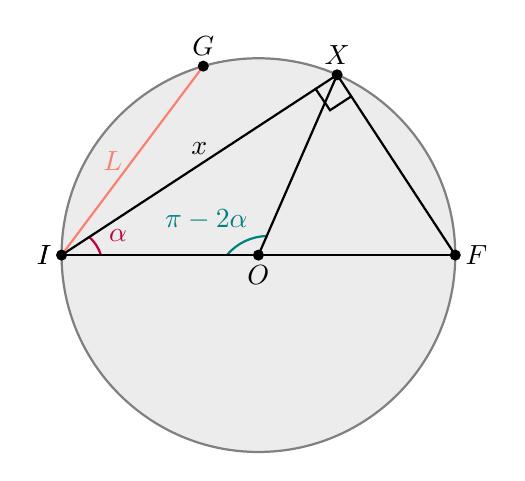
\begin{tikzpicture}[thick]
	\draw [color=gray, fill=gray!15] circle(2.5cm);
	\draw (0,0) coordinate [label= below:$O$] (D);
	\draw[color=teal] (0:-0.4) arc (140:90:0.68cm);
    \draw[color=teal] (-1.2cm:-0.8cm) node {$\pi - 2\alpha$};
    \draw[color=purple] (0:-2) arc (17:50:0.5cm);
    \draw[color=purple] (-8:-1.8) node {$\alpha$};
    \path[draw] (-2.5,0) coordinate [label= left:$I$] (A)
            -- node [above] {$x$} (1,2.29)  coordinate [label=above:$X$] (B)
            -- ( 2.5,0)  coordinate [label=right:$F$] (F);
    \path[draw] (0.72,2.12) -- (0.91, 1.84) -- (1.17, 2.01);
    \path[draw] (B) -- (D);
    \draw (-0.7,2.4) coordinate [label= above:$G$] (G);
    \path[draw, color=Salmon] (A) -- node [left] {$L$} (G);
    \path[draw] ( 2.5,0)  coordinate (F)
            -- (-2.5,0) coordinate [label= left:$I$] (A);
    \foreach \point in {A,B,D,F,G}
           \fill [black] (\point) circle (2pt);
\end{tikzpicture}
\end{minipage}
\begin{minipage}{0.64\textwidth}
	Пусть $I$ — точка, куда приземлился Илон Маск, а $G$ — точка, куда приземлилась Грета Тунберг.

	Так как точки, куда приземлились ребята, выбираются судьбой независимо, мы можем зафиксировать $I$ и менять только~$G$.

	Так как координата Греты распределена равномерно, то при допустимых значениях $x$:
	\[
  F_L (x) = \P(L \le x) =\P(\breve{IG} \le \breve{IX}) = \frac{\breve{IX}}{\breve{IF}} = \frac{r \cdot (\pi - 2\alpha)}{\pi r} 
  \]
\end{minipage}

  Угол $\alpha$ лежит в диапазоне $[0;\pi/2]$, поэтому:
	\[
  \cos \alpha = x \Rightarrow \alpha = \arccos x \Rightarrow F_L (x) = \frac{\pi - 2\arccos x}{\pi},
  \]

  В результате получаем плотность:
  \[
  f_L(x)
	= \begin{cases}
	\frac{2}{\pi \sqrt{1-x^2}}, \text{ если } x \in [0,1] \\
	0, \text{ иначе}
	\end{cases}
	\]
  Можно обойтись без производной арккосинуса, считая маленький участок окружности похожим на прямую, по мотивам
  \url{https://mrchasemath.com/2017/04/03/derivatives-of-trigonometric-functions/}.


  Мы рассмотрели только верхнюю часть Луны. 
  Если мы будем рассматривать возможность копать туннель также в нижней части Луны, 
  то в дроби $\P(L \le x) = \frac{\breve{IX}}{\breve{IF}}$ нам нужно будет удвоить и числитель, 
  и знаменатель. Отношение, которое мы ищем, не изменится, следовательно, не изменится вероятность.


	В случае объёмной Луны мы будем искать отношение площадей поверхностей.

	Илон Маск сидит в центре некоторой поляны Луны.
	Она образована точками, до которых туннель~$L$ не длиннее $x$. Для $x \in [0;1]$ получаем:
	\[
	F_L (x) = \P(L \le x) = \frac{\text{площадь поляны}}{\text{площадь поверхности сферы}} = \frac{2\pi r x^2}{4\pi r^2} = \frac{x^2}{2r} = x^2
	\]

  Тогда 
  \[
  f_L(x)= \begin{cases}
	2x, \text{ если } x \in [0,1] \\
	0, \text{ иначе} \\
  \end{cases}
  \]
  \item xxx
  \item xxx
\end{enumerate}



\subsection[2018-2019]{\hyperref[sec:kr_01_ip_2018_2019]{2018-2019}}
\label{sec:sol_kr_01_ip_2018_2019}

\begin{enumerate}

\item Воспользуемся методом первого шага. Дерево игры выглядит так (в вершинах — длительность сответствующей подыгры, а на концах ветвей — доля разбавленных пинт среди тех, что Джо помнит):
\begin{center}
\begin{tikzpicture} \node {$a$} child {node {1} edge from parent node[left] {Р} node[right] {}}
child {node {$b$}
child {node {1/2} edge from parent node[left] {Р}}
child {node (x) {$c$}
child {node (y) {$d$}
child {node (s) {$e$}
child {node {2/3} edge from parent node[right] {Р}}
edge from parent node[left] {НР}}
child {node {2/3} edge from parent node[right] {Р}}
edge from parent node[right] {Р}}
edge from parent node[right] {НР}}
edge from parent node[right] {НР}};
\draw [->,black] (x) .. controls +(down:1cm) and +(left:1cm) .. node[below,sloped] {НР} (x);
\draw [->,black] (s) .. controls +(up:0.1cm) and +(left:2.5cm) .. node[below,sloped] {НР} (x);
\end{tikzpicture}
\end{center}

Если первая пинта разбавлена, то игра заканчивается (разбавлены 100\% рома).
Если первая пинта не разбавлена, то, если разбавлена вторая, игра заканчивается (50\%).
Если вторая не разбавлена, и третья тоже, то это равносильно тому, что не разбавлены только две (Джо не помнит больше трех).
Если вторая не разбавлена, а третья разбавлена, возможны три случая: если четвёртая разбавлена, то игра заканчивается;
если четвёртая не разбавлена, и пятая не разбавлена, то это эквивалентно тому, что не разбавлены только две;
если четвёртая не разбавлена, а пятая разбавлена, то игра заканчивается.
Из этих соображений получаем систему уравнений:
\[
\begin{cases}a=\frac{1}{8}+\frac{7}{8}(b+1)\\
b=\frac{1}{8}+\frac{7}{8}(c+1)\\
c=\frac{1}{8}(d+1)+\frac{7}{8}(c+1)\\
d=\frac{1}{8}+\frac{7}{8}(e+1)\\
e=\frac{1}{8}+\frac{7}{8}(c+1)
\end{cases}
\]

Отсюда $a=7514/192,b=1046/24,c=146/3,d=122/3,e=136/3$.

\item Пусть
\[
Z_i=\begin{cases}1, i \mbox{-я пинта разбавлена} \\
0, \mbox{иначе}
\end{cases}
\]

Пусть с вероятностью $x_n$ последовательность случайных величин $(Z_n)$ длиной
$n$ не содержит двух единиц подряд и оканчивается нулём, а с вероятностью $y_n$ —
не содержит двух единиц подряд и оканчивается единицей.

Пусть на последнем месте $(Z_n)$ стоит единица. Это может произойти с вероятностью
$1/2$. При этом перед последней единицей может стоять любая последовательность
длиной $n-1$, оканчивающаяся нулём. Значит, $y_n=0.5x_{n-1}$.

Пусть на последнем месте $(Z_n)$ стоит нуль. Это может произойти с вероятностью
$1/2$. При этом перед последним нулём может стоять любая последовательность длиной
$n-1$. Значит, $x_n=0.5(x_{n-1}+y_{n-1})$.

Таким образом, получена следующая разностная система:
\[
\begin{cases}
x_n=0.5(x_{n-1}+y_{n-1})\\
y_n=0.5x_{n-1}
\end{cases}
\]

Более того, можно поставить задачу Коши. Так как $(Z_2)$ может равновероятно
иметь одну из 4 реализаций $(11, 10, 01, 00)$, из которых не содержат двух единиц
подряд и оканчиваются на 0 две, то $x_2=1/2$. Аналогично, $y_2=1/4$. Решив задачу
Коши, найдем формулы для $x_n$, $y_n$. Ответом будем число $x_{100}+y_{100}$.

\item
\begin{enumerate}
\item Оптимальная стратегия для Али-Бабы состоит в чередовании открытия двух
диагонально противоположных и двух соседних монет.

Изначально имеется только четыре варианта расположения монет:
\begin{center}
\begin{tikzpicture}[every node/.style={draw}]
\path[yshift=1.5cm,rectangle] (-6,0) node(a1){О} (-5,0) node(a2){Р} (-5,1) node(a3){О} (-6,1) node(a4){О};
\filldraw[fill=black] (a1) -- (a2) -- (a3) -- (a4) -- (a1);
\path[yshift=1.5cm,rectangle] (-4,0) node(a1){Р} (-3,0) node(a2){Р} (-3,1) node(a3){О} (-4,1) node(a4){О};
\filldraw[fill=black] (a1) -- (a2) -- (a3) -- (a4) -- (a1);
\path[yshift=1.5cm,rectangle] (-2,0) node(a1){Р} (-1,0) node(a2){О} (-1,1) node(a3){Р} (-2,1) node(a4){О};
\filldraw[fill=black] (a1) -- (a2) -- (a3) -- (a4) -- (a1);
\path[yshift=1.5cm,rectangle] (0,0) node(a1){Р} (1,0) node(a2){Р} (1,1) node(a3){Р} (0,1) node(a4){О};
\filldraw[fill=black] (a1) -- (a2) -- (a3) -- (a4) -- (a1);
\end{tikzpicture}
\end{center}

На первом ходе Али делает двух орлов на одной диагонали. Всего возможно восемь
случаев (по две диагонали в каждом из начальных вариантов). Из восьми равновозможных
случаев два приводят к успеху. При этом, если успех не достигнут, можно получить в
итоге только две комбинации орлов и решек (левую — в четырёх случаях, правую — в двух):
\begin{center}
\begin{tikzpicture}[every node/.style={draw}]

\path[yshift=1.5cm,rectangle] (-2,0) node(a1){О} (-1,0) node(a2){Р} (-1,1) node(a3){О} (-2,1) node(a4){О};
\filldraw[fill=black] (a1) -- (a2) -- (a3) -- (a4) -- (a1);
\path[yshift=1.5cm,rectangle] (0,0) node(a1){Р} (1,0) node(a2){О} (1,1) node(a3){Р} (0,1) node(a4){О};
\filldraw[fill=black] (a1) -- (a2) -- (a3) -- (a4) -- (a1);
\end{tikzpicture}
\end{center}

На втором ходе Али переворачивает две соседние монеты орлами вверх. При этом либо
наступает успех (8 случаев из 24), либо неуспех, приводящий к единтсвенно возможной
комбинации орлов и решек:
\begin{center}
\begin{tikzpicture}[every node/.style={draw}]
\path[yshift=1.5cm,rectangle] (-2,0) node(a1){О} (-1,0) node(a2){Р} (-1,1) node(a3){О} (-2,1) node(a4){О};
\filldraw[fill=black] (a1) -- (a2) -- (a3) -- (a4) -- (a1);
\end{tikzpicture}
\end{center}

На третьей попытке открывается или диагональ с орлами, или диагональ с орлом и решкой. В
о втором случае, очевидно, надо заменить решку на орла, и успех обеспечен. Но в первом
случае оптимально перевернуть орла и сделать 2 решки. Это даст неуспех, но Али точно
будет знать, что на четвёртой попытке монеты могут быть расположены только так:
\begin{center}
\begin{tikzpicture}[every node/.style={draw}]
\path[yshift=1.5cm,rectangle] (-2,0) node(a1){Р} (-1,0) node(a2){Р} (-1,1) node(a3){О} (-2,1) node(a4){О};
\filldraw[fill=black] (a1) -- (a2) -- (a3) -- (a4) -- (a1);
\end{tikzpicture}
\end{center}

На четвёртом ходе в любом из четырёх вариантов (Али не знает, на каком ребре решки)
нужно перевернуть обе открытые соседние монеты, тогда в двух случаях будет успех,
а в двух других -- неуспех, при котором монеты могут быть расположены только так:
\begin{center}
\begin{tikzpicture}[every node/.style={draw}]
\path[yshift=1.5cm,rectangle] (-2,0) node(a1){Р} (-1,0) node(a2){О} (-1,1) node(a3){Р} (-2,1) node(a4){О};
\filldraw[fill=black] (a1) -- (a2) -- (a3) -- (a4) -- (a1);
\end{tikzpicture}
\end{center}

Очевидно, что если на пятом ходе, открыв любую диагональ, Али перевернёт находящиеся
на ней монеты, то он гарантирует себе успех.

\item Как видим, в худшем случае потребовалось $5$ попыток.
\end{enumerate}
Источник: Кордемский, Математика изучает случайности.

\item Возьмём колоду, добавим в неё джокера. Разложим в открытую по окружности.
Джокер означает место разрыва окружности для её выкладывания в обычную колоду.
Замечаем, что джокер и четыре дамы разбивают окружность на пять случайных отрезко.
В силу симметрии ожидаемые длины этих отрезков равны и равны по $48/5$.
Значит первая дама попадается в среднем на $48/5 + 1$ месте.

\item Обозначим искомую вероятность быть в Неведении в момент $t$ значком $p_t$.
\[
p_{t+\Delta} = p_t (1-\lambda\Delta - o(\Delta))
\]

Отсюда получаем, что
\[
\frac{p_{t+\Delta} - p_t}{\Delta} = -\lambda p_t + \frac{o(\Delta)}{\Delta}
\]
Устремляем $\Delta$ к нулю и решаем получающееся дифференциальное уравнение
с начальным условием $p_0 = 1$, так как изначально Ученик находится в Неведении.

Итого:
\[
p_t = \exp(-\lambda t)
\]

\item
\[
\P(Y_4 \in [t; t+\Delta]) = C_{10}^1 \cdot \Delta \cdot C_{9}^3 t^3 (1-t)^6 + o(\Delta)
\]

Читаем вслух:
\begin{enumerate}
  \item Одна из десяти величин должна попасть в отрезок $[t; t + \Delta]$;
  \item Три из девяти оставшихся должны оказаться меньше $t$;
  \item Шесть из девяти оставших должны оказаться больше $t$;
\end{enumerate}
Вероятностью попадания двух и более величин в отрезок длины $\Delta$ пренебрегаем!
\end{enumerate}

\subsection[2017-2018]{\hyperref[sec:kr_01_ip_2017_2018]{2017-2018}}
\label{sec:sol_kr_01_ip_2017_2018}

\begin{enumerate}
\item Обозначим вероятность того, что сыр достанется Белому за $b$, если игра
начинается с его броска.

\begin{enumerate}
\item Получаем уравнение
\[
b = \frac{1}{12} + \frac{11}{12} \cdot \frac{11}{12} b
\]

Пояснение: Как Белый может победить в исходной игре? Либо сразу выкинуть 6 с вероятностью $1/12$.
Либо передать ход Серому ($11/12$), получить ход снова ($11/12$) и выиграть в продолжении игры.
Продолжение игры по сути совпадает с исходной игрой.

\item Игра продолжается до тех пор, пока кто-то не выкинет «6».
Для нахождения среднего количества бросков воспользуемся методом первого шага.

Обозначим среднее количество бросков нашей игры за $S$.
Когда Белый бросает кубик, с вероятностью $\frac{1}{12}$ игра закончится за один бросок,
а с вероятностью $\frac{11}{12}$ игра продолжится и ход перейдёт к Серому.
Но та игра, которая начнётся, когда бросать будет Серый, ничем не отличается от предыдущей,
поэтому среднее количество бросков в ней будет равно $S$.
Однако мы попадём в эту игру, «потратив» один бросок. Таким образом мы получаем:

\[
S = \frac{1}{12} \cdot 1 + \frac{11}{12}(S +1)
\]

Получается, что $S = 12$, значит игра длится в среднем 12 бросков.
\end{enumerate}

\item

\item Для того, чтобы выжить, мышам нужно ещё до начала игры договориться о стратегии,
которая позволит им с наибольшей вероятностью открыть нужные сундуки.
Если хотя бы две мыши выберут одинаковый сундук, то их в любом случае съедят.
Поэтому одной из оптимальных стратегий будет ещё до начала игры мышам договориться
и назвать левый сундук золотым, сундук посередине серебряным, а правый — платиновым.
Каждый мышонок должен открыть тот сундук, в честь которого назван необходимый ему металл.
Если внутри он обнаруживает свой металл, то он выбирает этот сундук,
если внутри находится не тот металл, мышонок открывает тот сундук,
на который указывает лежащий внутри предмет.

Например, первым заходит Микки Маус. Он открывает золотой (левый) ящик.
Если внутри лежит золото, то он выходит из комнаты. Если же внутри лежит, например, серебро,
то Микки Маус открывает сундук посередине.
Путём перебора можно посчитать, что в 4 случаях из 6 мыши смогут найти нужный металл,
поэтому вероятность выигрыша при данной стратегии равна $\frac{2}{3}$.

\item
\begin{enumerate}
  \item Обозначим буквой $X$ количество детей в случайной семье.
  Можно просуммировать ряд $\E(X) = 1\cdot 0.5 + 2\cdot 0.5^2 + 3\cdot 0.5^3 + \ldots$. 
  А можно воспользоваться методом первого шага и заметить, что либо первой рождается девочка 
  и мышиная семья больше не заводит мышат, либо рождается мальчик и семья ситуация превратилась в первоначальную
  плюс один ребёнок.

  \[
  \E(X) = 0.5 \cdot 1 + 0.5 \cdot (1 + \E(X))  
  \]
  Находим, $\E(X)=2$.
  \item В мышиной стране много семей. Занумеруем семьи. Обозначим буквой $X_i$ число детей в $i$-ой семье.
  Тогда доля $D$ — это суммарное количество мальчиков делить на суммарное количество детей:

  Получаем
  \[
  \frac{(X_1 - 1) + (X_2 - 2)+ \ldots + (X_n - 1)}{X_1 + X_2 + \ldots +X_n} = 1 - \frac{n}{\sum_{i=1}^n X_i}  
  \]

  Основной смысл математического ожидания $\E(X_i)$ — это среднее выборочное при большом количестве повторений опыта.

  Следовательно, $\frac{\sum_i X_i}{n} \to \E(X_i)=2$. И стало быть, при $n\to\infty$ получаем $D \to 1 - 1/2=1/2$.

  Интуитивный аргумент немного опасен, но всё же приведём его: вероятности рождения мальчиков и девочек равны,
  поэтому и доля будет половина. 
  Опасность аргумента состоит в том, что семьи могли бы в альтернативном условии рожать мышат по принципу: 
  пока доля мальчиков в стране не превысит 50\%. 

  \item Можно просто аккуратно суммировать ряд:
  \[
  \E(Y) = 0.5 \cdot \frac{0}{1} + 0.5^2 \cdot \frac{1}{2} + 0.5^3 \cdot \frac{2}{3} + \ldots
  \]

  Здесь мудрый студент может вспомнить ряд Тейлора для логарифма:
  \[
  \ln (1 + r) = r - r^2/2 + r^3/3 - r^4/4 +\ldots
  \]

  Стало быть,
  \[
  \ln (1 - 0.5) = -0.5 - 0.5^2/2 - 0.5^3/3 - 0.5^4/4  +\ldots 
  \]

  И исходное ожидание равно:

  \[
  \E(Y) = 1 + \ln 0.5 = 1 - \ln 2 \approx 0.31  
  \]

\item Неожиданно лёгкий вопрос, $\E(X - 1) = 2 -1=1$.
\end{enumerate}


\item Благосостояние кота Василия, положившего один гурд на вклад,
равно $m_t = 1\cdot e^{rt}$, где $r$ — процентная ставка, а $t$ — прошедшее время.

Откуда взялась экспонента?

Допустим время дискретно, а процентная ставка равна 5\% в год. 
Тогда сумма вклада каждый год домножается на $1.05$ и эволюционирует по формуле:

\[
m_t = 1 \cdot 1.05^t
\]

Но любое число можно представить в виде экспоненты, $1.05 = e^{\ln 1.05}$.

Поэтому
\[
m_t = e^{\ln 1.05 \cdot t}  = e^{rt}
\]


Момент закрытия вклада $T$ равномерно распределён на отрезке от 0 до $a$,
поэтому сумма, которую получит Василий, представима в виде $Z = e^{Y}$, где $Y \sim U[0; ra]$.
По условию, $a$ очень велико, поэтому $ra$ тоже очень велико.

Вероятность того, что первая цифра будет равна 1, равна вероятности того,
что доход Василия будет лежать в пределах от 1 до 2 гурдов, плюс вероятность того,
что он лежит в пределах от 10 до 20 гурдов и т.д.
Таким образом, можно представить эту вероятность, как:
\[
\P(N=1) = \P(e^Y \in [1;2) ) + \P(e^Y \in [10; 20) ) + \ldots
\]

Это выражение можно преобразовать таким образом:
\[
\P(N=1) = \P(Y \in [\ln 1; \ln2) ) + \P(Y \in [\ln 10; \ln 20) ) + \ldots
\]

Так как $Y$ — равномерно распределённая величина,
то $\P(Y \in [\ln 1; \ln2) ) = \frac{\ln 2 - \ln 1}{ra}$.
Для последующих слагаемых вероятность рассчитывается таким же образом.
Воспользовавшись свойством логарифма, можно заметить,
что $\frac{\ln 20 - \ln 10}{ra} = \frac{\ln 2}{ra}$.
Поэтому вероятность того, что на первом месте суммы вклада стоит единица,
равна $n\cdot \frac{\ln 2}{ra}$, где $n$ — количество слагаемых.
Путём аналогичных рассуждений получаем, что вероятность того,
что на первом месте стоит двойка, равна $n\cdot \frac{\ln 3- \ln 2}{ra}$.
Из-за того, что $a$ велико, можно считать, что число слагаемых одинаково.

На первом месте обязательно будет находиться какая-то цифра,
поэтому сумма вероятностей будет равна 1. Получаем:
\[
\frac{n}{ra}\left(\ln \frac{2}{1} + \ln \frac{3}{2} + \ldots + \ln \frac{10}{9}\right) = 1
\]

Таким образом $\frac{n}{ra} = \frac{1}{\ln 10}$.
Получается, что вероятность того, что на первом месте стоит единица, равна:
\[
\P (N=1) = \frac{\ln 2}{\ln 10}
\]

Закон распределения первой цифры выводится сложением соответствующих вероятностей.
\end{enumerate}


\subsection[2016-2017]{\hyperref[sec:kr_01_ip_2016_2017]{2016-2017}}
\label{sec:sol_kr_01_ip_2016_2017}

\begin{enumerate}
\item
\begin{enumerate}
\item Для удобства занумеруем макаронины и выделим у каждой левый и правый конец.
Взяли правый конец первой макаронины и подвязали случайной.
Взяли свободный конец только что подвязанной макаронины и подвязали случайно. И так далее.
\[
\frac{2n-2}{2n-1}\cdot \frac{2n-4}{2n-3}\cdot \ldots \cdot \frac{2}{3} \cdot 1
\]
\item Допустим, что при $n$ макаронинах в среднем образуется $e_n$ колец.
После первого соединения задача сводится к меньшему числу макаронин, важно только учесть,
образовалось ли кольцо при первом соединении:
\[
e_n = \frac{1}{2n-1}(e_{n-1}+1) + \frac{2n-2}{2n-1}e_{n-1} = e_{n-1} + \frac{1}{2n-1}
\]
\item Количество коротких колец можно разбить в сумму, $X=Z_1 + \ldots + Z_n$.
Вероятность завязывания конкретной макаронины в кольцо равна $1/(2n-1)$:
«левый конец» надо привазять именно к «правому». Значит, $\E(X)=n/(2n-1)$.
\end{enumerate}

\item
\begin{enumerate}
\item Рассмотрим обратную ситуацию: на планете есть точка, из которой связаться
хотя бы с одним пепелацем нельзя. Такое возможно, если все, кроме одного, сели
в одну полуокружность.
\[
\P(\text{есть точка без связи}) = n \cdot \left(\frac{1}{2}\right)^{n-1}
\Rightarrow \P(\text{из любой точки есть связь}) =
1 - n \cdot \left(\frac{1}{2}\right)^{n-1}
\]
\item Зафиксируем координату посадки первого пепелаца и возьмём её за точку отсчёта.
Изобразим на плоскости возможные значения центральных углов между первым пепелацем и
оставшимися и закрасим нужные участки. Получим $3/8$.
\item Зафиксируем координату посадки первого пепелаца. Обозначим центральный угол
между первым и вторым пепелацами $\alpha$. Функция плотности имеет вид:
$p(\alpha) = \frac{\sin \alpha}{2}$

Итог: $\int_0^{\pi/2} p(\alpha) \frac{\alpha + \pi}{2\pi} d \alpha + \int_{\pi/2}^{\pi}
p(\alpha) \frac{\pi - \alpha}{2\pi} d \alpha = \frac{\pi + 2}{4\pi}$
\end{enumerate}

\item Вспомним для начала, что площадь круга равна $\pi r^2$, а площадь сферы равна
$4\pi r^2$. Составим из маленьких треугольничков многогранник очень похожий на сферу
с единичным радиусом. Площадь этого многогранника будет примерно равна $4\pi$.
Проекция многогранника представляет собой примерно круг единичного радиуса.
Проекция имеет два слоя. С учётом обоих слоёв площадь проекции равна $2\pi$.
Значит отношение площади проекции к площади многогранника равно $1/2$.

От взаимного расположения треугольничков в пространстве ожидаемая площадь
проекции не зависит в силу аддитивности математического ожидания.

Ответ: 21 см$^2$.

\item
\begin{enumerate}
\item Мысленно отметим на окружности три точки: места ударов Брюса Ли и точку,
где схватился Чак Норрис. Можно считать, что эти три точки равномерно и независимо
распределены по окружности. Следовательно, среднее расстояние между соседними
точками равно $1/3$. Чак Норрис берёт два кусочка, слева и справа от своей точки.
Значит ему в среднем достаётся $2/3$ окружности.
\item Объявим точку, где схватился Чак Норрис нулём. Координаты двух ударов
изобразим на плоскости. Закрашиваем подходящий участок. Вероятность того, что
кусок Брюса Ли длиннее, равна $1/4$.
\end{enumerate}

\item  Рассмотрим совершенно конкурентный невольничий рынок начинающих певиц.
Певицы в хорошем настроении продаются по $V_1$, в депрессии — по $V_2$.
Получаем систему уравнений:
\[
\begin{cases}
  V_1 = 0.75 + (0.5 V_1 + 0.5 V_2) \\
  V_2 = \max_x \sqrt{x}V_1 + (1 - \sqrt{x})V_2 - x
\end{cases}
\]
Оптимизируем и получаем, $x^* = (V_1 - V_2)^2/4$. Из первого уравнения находим
$(V_1 - V_2)/2=0.75$.

\item Да. Например, такая. До общения с Джульеттой подкидывать монетку до выпадения
первого орла и запомнить число потребовавшихся подбрасываний. Пусть это будет число $X$.
Открыть равновероятно левую или правую руку Джульетты. Если открытое число больше $X$,
то сказать, что оно большее, иначе сказать, что меньшее.
\item Если $\gamma$ — вероятность самостоятельного познания Истины, а $\alpha$ —
передачи Истины отдельно в каждую из сторон, то
\[
p = \gamma + (1-\gamma) p \alpha.
\]

То есть $p=\gamma/(1-\alpha(1-\gamma))$.

Для решения второго пункта наложим на Абу Али Хусейн ибн Абдуллах ибн аль-Хасан
ибн Али ибн Сина обет молчания. Это не повлияет на вероятность постижения им Истины,
однако превратит задачу в две уже решённых :) Получаем
\[
q = \gamma + (1-\gamma)(2p\alpha - p^2\alpha^2)
\]
\end{enumerate}



\subsection[2015-2016]{\hyperref[sec:kr_01_ip_2015_2016]{2015-2016}}
\label{sec:sol_kr_01_ip_2015_2016}

\subsubsection*{Индивидуальный тур}

\begin{enumerate}
\item Сократ, эта — Η, η, дзета — Ζ, ζ, вега — нет, шо — ϸ, τ — тау, θ — тета, ξ — кси.
Греческая буква шо, ϸ, была введена Александром Македонским и ныне вышла из употребления.
По крайней мере, в греческом :) Заглавная примерно такая же, только её utf-код 03f7
не поддерживается шрифтом Linux Libertine.

\item Да. Cобытия независимы в совокупности, если для любого поднабора событий $A_1$,
\ldots, $A_k$ выполняется равенство $\P(A_1 \cap A_2 \cap \ldots \cap A_k) = \P(A_1)
\cdot \ldots \cdot \P(A_k)$. Нет.
\item $1/4$, $2/3$, $15$
\item $0$, $0.8^5\cdot 0.2$, $1-0.8^6$
\item $0.8^{10}$, $C_{10}^3 0.2^3 0.8^7$, $2$
\item $1/2$, $3/16$, $3/8$
\item
\begin{enumerate}
\item
\begin{flalign*}
F_X(x) &= \begin{cases}
0, \, x<0 \\
x^3, \, x \in [0;1] \\
1, \, x>1
\end{cases}&&
\end{flalign*}
\item $1/8$
\item $2^{-1/3}$
\item $56/63$
\item
\begin{flalign*}
F_Y(y) &= \begin{cases}
0, \, y<0 \\
1-1/y^3, \, y>0
\end{cases}&&
\end{flalign*}
\item
\begin{flalign*}
f_Y(y) &= \begin{cases}
0, \, y<0 \\
3y^{-4}, \, y>0
\end{cases}&&
\end{flalign*}

\end{enumerate}
\end{enumerate}

\subsubsection*{Командный тур}

\begin{enumerate}
\item Если отрублено 10 щупалец, значит либо был один удар породивший два новых
щупальца, либо было два удара, породивших по одному новому, а все остальные удары
не порождали новых щупалец.

Искомая вероятность равна: $8\cdot 0.5^9 \cdot 0.25^1 + C_8^2 0.5^8 0.25^2$.

Вероятность вечного боя равна нулю. Достаточно доказать, что с вероятностью один
за конечное время побеждается одноногий Кракен. А эта вероятность удовлетворяет
уравнению: $p=\frac{1}{4}p + \frac{1}{4}p^2 + \frac{1}{2} 1$. Единственный осмысленный
корень у этого уравнения — $1$.

Замечаем, что на победу над $k$-шупальцевым Кракеном уходим в $k$ раз больше ударов
в среднем чем на победу на $1$-щупальцевым. Отсюда:
\[
e_1=1 + 0.5\cdot 0 + 0.25\cdot e_1 + 0.25 \cdot 2e_1
\]
Решаем, получаем $e_1=4$ и $e_8=32$

\item Либо первая пинта разбавлена, либо первая неразбавлена, а вторая разбавлена,
то есть
\[
0.25 + 0.75\cdot 0.25 =0.4375
\]
Рисуем граф. %:

Составляем систему (индекс — количество выпитых неразбавленных пинт):
\[
\begin{cases}
e_0=\frac{1}{4} + \frac{3}{16}2 + \frac{9}{16}(2+e_2) \\
e_2=1+\frac{3}{4}e_2 + \frac{1}{4}e_0
\end{cases}
\]
Находим $e_0=64/7\approx 9$

\item Для $t>0$:
\[
\P(-\ln X \leq t)=\P(\ln X > -t)=\P(X > e^{-t})=1-e^{-t}
\]
Итого,
\[
F_{-\ln X}(t)=\begin{cases}
0, \, t < 0 \\
1-e^{-t}, \, t \geq 0
\end{cases}
\]
Из геометрических соображений легко найти $\P(XY < a)$ для $a\in (0;1)$:
\[
\P(XY < a)=a + \int_a^1 \frac{a}{x} \, dx=a-a\ln a
\]
Переходим ко второму пункту, для $t>0$:
\[
\P(-(\ln X + \ln Y) < t)=\P(XY > e^{-t})= 1-e^{-t} -t e^{-t}
\]
Итого:
\[
F_{-\ln X - \ln Y}(t)=\begin{cases}
0, \, t < 0 \\
1-e^{-t} - te^{-t}, \, t \geq 0
\end{cases}
\]
После дифференциирования получаем функцию плотности для $S=-\ln X - \ln Y$:
\[
f_S(s)=\begin{cases}
0, \, s < 0 \\
se^{-s}, \, s \geq 0
\end{cases}
\]
Приближаемся к финальной вероятности:
\[
\P(ZS > t)= \int_t^{\infty} \int_{t/s}^1  se^{-s} \, dz\, ds=
\int_t^{\infty} (s-t)\cdot e^{-s} \, ds= \ldots = e^{-t}
\]
Сравниваем результат с первым пунктом и приходим к выводу, что величина $(XY)^Z$
имеет равномерное распределение на $[0;1]$.

\item Если нанято $n$ пиратов, то вероятность, того, что в конкретный день все
работают равна $(364/365)^n$. Следовательно, ожидаемое количество праздничных дней
равно $365(1-(364/365)^n)$.

Решаем уравнение:
\[
1-(364/365)^n=100/365
\]
Получаем:
\[
n=\frac{\ln 265- \ln 365}{ \ln 364 - \ln 365}\approx 117
\]
Ожидаемое количество рабочих пирато-дней равно: $365n(364/365)^n$.

Получаем:
\[
n^*=1/(\ln 365 - \ln 364)\approx 364
\]

\item
\begin{enumerate}
\item $\P(R_{100})=1/100$ (максимум из 100 величин должен плюхнуться на сотое место),
$\P(B_{100})=1/3$ (максимум из трёх величин должен плюхнуться на второе место)
\item $X=X_1+X_2+\ldots + X_{100}$ и $\E(X_i)=1/i$, поэтому:
\[
\E(X)=1+\frac{1}{2} + \frac{1}{3}+\ldots + \frac{1}{100}\approx \ln 100 \approx 4.6
\] 
\item $\P(R_{99} | R_{100})=1/99$, $\P(R_{100}|B_{100})=3/101$

Для проверки: $\P(R_{99} \cap R_{100})=98!/100!$ ($100!$ — всего перестановок,
$98!$ — первые 98 можно переставлять свободно, а в конце должны идти второй
наибольшое и наибольшее). $\P(R_{100} \cap B_{100})=1/101$ (максимум из 101 числа
плюхнется на 100ое место).
\end{enumerate}

\item Если все пираты открывают первый и второй сундуки, то вероятность выигрыша
равна нулю.

Оптимальная стратегия (одна из). Три пирата заранее договариваются, о названиях сундуков.
Они называют эти три сундука (ещё до игры)  «рубиновым», «пиастровым» и «золотым».
Генри Рубинов должен начать с открытия рубинового сундука, Френсис Пиастров —
с пиастрового, Эдвард Золотов — с золотого. Далее каждый пират должен открыть тот
сундук, на который указывает предмет, лежащий в первом открытом им сундуке. Например,
если Генри Рубинов, открыв сначала рубиновый сундук обнаруживает там пиастры, он должен
открывать пиастровый сундук.

Вероятность победы при такой стратегии легко находится перебором 6 возможных вариантов
и равна\ldots Та-дам!!! $2/3$.
\end{enumerate}


\subsection[2014-2015]{\hyperref[sec:kr_01_ip_2014_2015]{2014-2015}}
\label{sec:sol_kr_01_ip_2014_2015}


\subsubsection*{Часть 1}

Не претендуя на единственность, решения претендуют на правильность!

\begin{enumerate}
\item
\begin{enumerate}
\item $\P(\text{все арбузы спелые}) = 0.9^2\cdot 0.7 = 0.567  $
\item $A$ = \{случайно выбранный арбуз — от тёти Маши\};
$B$ = \{случайно выбранный арбуз оказался спелым\}. Формула условной вероятности:
\[
\P(A|B) = \frac{\P(A \cap B)}{\P(B)} = \frac{2/3 \cdot 0.9}{2/3 \cdot 0.9 + 1/3 \cdot 0.7}
= \frac{18}{25}
\]
\item $A$ = \{второй и третий съеденные арбузы — от тёти Маши\};
$B$ = \{все три арбуза — спелые\}. Дает ли нам что-то о принадлежности арбузов
к тёте Маше или тёте Оле то, что все арбузы — спелые? События независимы!
\[
\P(A|B) = \P(A) = \frac{1}{3}
\]
\end{enumerate}

\item
\begin{enumerate}
\item $\E(X) = \sum \P(X_i) X_i = 1.9$

$\Var(X) = \E(X^2) - (\E(X))^2 = 0\cdot 0.1 + 1 \cdot 0.3 + 4 \cdot 0.2 +
9 \cdot 0.4 - 1.9^2 = 1.09$

\item Раз ребенок выбран, значит, в его семье дети есть! Всего детей $n\E(X) = 1.9n$.
Семей с одним ребенком — $0.3n$, значит, детей из семей с одним ребенком — $0.3n$.
Аналогично, детей из семей с двумя детьми — $0.4n$; детей из семей с тремя детьми — $1.2n$.

Теперь легко построить закон распределения случайной величины $Y$:

\begin{center}
\begin{tabular}{cccc}
\toprule
$y$ & $1$ & $2$ & $3$  \\
$\P(Y=y)$ & $3/19$ & $4/19$ & $12/19$  \\ \bottomrule
\end{tabular}
\end{center}

\[
\E(Y) = \frac{3}{19} + \frac{8}{19} + \frac{36}{19} = \frac{47}{19} > \E(X)
\]
\end{enumerate}

\item
Любителям (или нелюбителям) интегралов:
\begin{enumerate}
\item Да это же интеграл от функции плотности на всей числовой прямой! Ответ: единица!
\item \[
\E(X) = \int \limits_0^2 x f(x) dx = \int \limits_0^2 \frac{3}{8} x^3 dx =
\left. \frac{3}{32} x^4 \right|_0^2 = \frac{3}{2}
\]

\[
\E\left(X^2\right) = \int \limits_0^2 x^2 f(x) dx = \int \limits_0^2 \frac{3}{8} x^4 dx
= \left. \frac{3}{40} x^5 \right|_0^2 = \frac{12}{5}
\]

Формула дисперсии:
\[
\Var(X) = \E\left(X^2\right) - \left(\E(X) \right)^2 = \frac{12}{5} - \frac{9}{4} = \frac{3}{20}
\]

\item \[
\P(X>1.5) = \int \limits_{1.5}^2 f(x) dx = \int \limits_{1.5}^2 \frac{3}{8} x^2 dx =
\left.\frac{1}{8} x^3 \right|_{1.5}^2 = \frac{37}{64}
\]

Вычислим вероятность условия:

\[
\P(X>1) = \int \limits_1^2 f(x) dx = \int \limits_1^2 \frac{3}{8} x^2 dx
= \left. \frac{1}{8} x^3 \right|_1^2 = \frac{7}{8}
\]

\[
\P(X>1.5 | X>1) = \frac{\P(X>1.5)}{\P( X>1)} = \frac{37/64}{7/8} = \frac{37}{56}
\]

\item Должно выполниться следующее соотношение:
\[
\int \limits_{-\infty}^{+\infty} c x f(x) dx  = 1
\]

Применительно к нашей задаче:
\[
\frac{3c}{8} \int \limits_0^2 x^3 dx  = \left.\frac{3c}{32} x^4 \right|_0^2 = \frac{3c}{2} =
1 \Rightarrow c = \frac{2}{3}
\]
\end{enumerate}

\item
You have to learn the rules of the game. And then you have to play better than
anyone else. (А. Эйнштейн)

\begin{enumerate}
\item \[
\Var(Z) = \E\left(Z^2\right) - (\E(Z))^2 = 15 - 9 = 6
\]
\[
\Var(4 - 3Z) = 9\Var(Z) = 54
\]
\[
\E\left(5 + 3Z - Z^2\right) = 5 + 3\cdot (-3)  - 15 = -19
\]

\item
\[
\Var(X \pm Y) = \Var(X) + \Var(Y) \pm 2 \cdot \Cov(X, Y)
\]
Отсюда получаем:
\[
\Var(X + Y) - \Var(X - Y) = 4 \Cov(X, Y) \Rightarrow \Cov(X, Y) = 2.5
\]
\[
\Cov(6 - X, 3Y) = -3\cdot 2.5 = -7.5
\]

\item
\[
\Cov(X, Y) = 2.5 \ne 0
\]
Случайные величины действительно независимы.
\end{enumerate}

\item
В условии не сказано сколько ответов являются верными. Предположим, что правильный
ответ $0.25$. Но это невозможно, потому что вариантов ответа $0.25$ — два (1 и 4),
значит ответ $0.5$ тоже был бы правильный. Предположим, что правильный $0.5$.
Тогда $0.25$ тоже правильный — таких вариантов два из четырех, значит вероятность
попасть в $0.25$, выбрав ответ наугад, равна $0.5$. Ответ $0.6$, очевидно, неверен,
потому что вероятность попасть в него равна $0.25$. \\
\textbf{Правильный ответ:} $0$

\item
Удобно рассуждать следующим образом: предположим, что каждая опечатка наугад
(с равными вероятностями и независимо от других опечаток) выбирает, на какую
страницу ей попасть\footnote[1]{Ну очень самостоятельные!}.

\begin{enumerate}
\item Пусть $X$ — число опечаток на 13 странице.
\[
\P(X \geqslant 2) = 1 - \P(X=0) - \P(X=1)
\]
$\P(X=0) = \left( \frac{499}{500} \right)^{400}$ — каждая из 400 опечаток
не доложна попасть на 13 страницу.

$\P(X=1) = 400\cdot\frac{1}{500}\cdot\left( \frac{499}{500} \right)^{399}$ —
ровно одна опечатка (а есть 400 вариантов) должна попасть на 13 страницу,
а остальные — мимо. Соответственно:
\[
\P(X \geqslant 2) = 1 - \left( \frac{499}{500} \right)^{400} -
400\cdot\frac{1}{500}\cdot\left( \frac{499}{500} \right)^{399} \approx 0.1911357
\]
Это если считать в явном виде. А если пользоваться приближением Пуассона:
\[
p(k) = \P(X = k) = \frac{\lambda^k}{k!}e^{-\lambda}
\]
неплохо бы вспомнить, что параметр $\lambda$ это математическое ожидание $X$,
поэтому расчеты здесь пока оставим до лучших времен.

\item Пусть $X$ — число опечаток на 13 странице. Введем случайную величину
\[
X_i =
\begin{cases}
1 & \text{если } i\text{-ая опечатка попала на 13 страницу}\\
0 & \text{если нет}
\end{cases}
\]
Тогда $X = \sum\limits_{i=1}^{400}X_i$. Рассмотрим отдельно $X_i$:

\begin{center}
\begin{tabular}{@{}ccc@{}}
\toprule
$x$         & $1$             & $0$               \\
$\P(X=x)$ & $\frac{1}{500}$ & $\frac{499}{500}$ \\ \bottomrule
\end{tabular}
\end{center}

Так как $i$-ая опечатка наугад выбирает одну страницу из 500 и это должна быть именно 13.

Тогда:
\[
\E(X_i) = \frac{1}{500} = \E(X^2_i) \Rightarrow
\]
\[
\Var(X_i) = \E(X^2_i) - (\E(X_i))^2 = \frac{1}{500} - \left(\frac{1}{500}\right)^2 = \frac{499}{500^2}
\]
Значит
\[
\E(X) = \E\left(\sum\limits_{i=1}^{400}X_i\right) = \sum\limits_{i=1}^{400}\E(X_i)  = \frac{400}{500} = 0.8
\]

\[
\Var(X) = \Var\left(\sum\limits_{i=1}^{400}X_i\right) = \sum\limits_{i=1}^{400}\Var(X_i) = 400\cdot\frac{499}{500^2} = 0.8\cdot\frac{499}{500}
\]

Теперь мы знаем, что $\lambda = \E(X) = 0.8$ поэтому можем вернуться к пункту (а):
\[
\P(X \geqslant 2) = 1 - \P(X=0) - \P(X=1)  = 1 - \frac{0.8^0}{0!}e^{-0.8} - \frac{0.8^1}{1!}e^{-0.8} = 0.1912079
\] \vspace{-1.2cm}

\hspace{13cm} \fcolorbox{ForestGreen}{white}{So close!}

Осталось найти наиболее вероятное число опечаток на 13 странице:
\[
\P(X=k) = \frac{0.8^k}{k!}e^{-0.8} \rightarrow \max \limits_k
\]
Очевидно, что эта функция убывает по $k$, ведь с ростом $k$:\\
 $k!$ растет, а $0.8^k$ убывает. Значит наиболее вероятное число ошибок — $X = 0$


\item \href{https://en.wikipedia.org/wiki/Triskaidekaphobia}{Ох уж эти предрассудки!}
13-я страница точно такая же как и все остальные, ведь везде в решении можно просто
заменить номер 13 на любой другой и ничего не изменится.
\begin{center}
\includegraphics[width=6cm]{images/13}
\end{center}
\end{enumerate}

\item
Пусть $A = \{\text{«Лекция полезна»}\}$, $B = \{\text{«Лекция интересна»}\}$.
Заметим, что лекции вообще независимы друг от друга.

\begin{enumerate}
\item Пусть $X_A$ — число полезных лекций, прослушанных Васей,  $X_B$ —
число интересных лекций, прослушанных Васей. Введем случайную величину:
\[X_i =
\begin{cases}
1 & \text{если } i\text{-ая лекция была полезна}\\
0 & \text{если нет}
\end{cases}
\]

Тогда $X_A = \sum\limits_{i=1}^{30}X_i$. Рассмотрим отдельно $X_i$:

\begin{center}
\begin{tabular}{@{}ccc@{}}
\toprule
$x$         & $1$             & $0$               \\
$\P(X=x)$ & $0.9$ & $0.1$ \\ \bottomrule
\end{tabular}
\end{center}

Вероятность $0.9$ дана. Тогда:
\[
\E(X_i) = 0.9 = \E(X^2_i) \Rightarrow
\]
\[
\Var(X_i) = \E(X^2_i) - (\E(X_i))^2 = 0.9 - 0.9^2 = 0.09
\]

Значит,
\[
\E(X_A) = \E\left(\sum\limits_{i=1}^{30}X_i\right) = \sum\limits_{i=1}^{30}\E(X_i)  =
0.9\cdot30 = 27
\]
\[
\Var(X_A) = \Var\left(\sum\limits_{i=1}^{30}X_i\right) = \sum\limits_{i=1}^{30}\Var(X_i) =
0.09\cdot30 = 2.7
\]

Аналогично для числа интересных лекций можем получить:
\[
\E(X_B) = 0.7\cdot 30 = 21
\]
\[
\Var(X_B) = 0.21\cdot 30 = 6.3
\]


\item Так как интересность и полезность — независимые свойства лекций, то:

$\P(\bar{A} \cap \bar{B}) = \P(\bar{A})\cdot \P(\bar{B}) = 0.3\cdot0.1 = 0.03$, где $\bar{A}$ значит «не $A$». В свою очередь:\\
 $\P(A\cup B) = \P(A\cap\bar{B}) + \P(B\cap\bar{A}) + \P(A\cap B) = 1 - \P(\bar{A})\cdot \P(\bar{B}) = 0.97$ , где $(A\cup B)$ значит «$A$  или $B$». Аналогично, путем введения бинарной случайной величины можем получить:
 \[
 \E(X_{\bar{A} \cap \bar{B}}) = 0.03 \cdot  30 = 0.9
 \]
 \[
 \E(X_{A\cup B}) = 0.97\cdot30 = 29.1
\]
\end{enumerate}

\item
Будем пользоваться свойствами функций распределения и плотности. Для начала:
\[
\lim\limits_{x \rightarrow +\infty} F(x) = 1, \hspace{0.5cm} \lim\limits_{x \rightarrow -\infty} F(x) = 0,
\]
\[
\lim\limits_{x \rightarrow +\infty} \left(\frac{ae^x}{1+e^x}+b\right) = a+b := 1
\]
\[
\lim\limits_{x \rightarrow -\infty} \left(\frac{ae^x}{1+e^x}+b\right) = b :=0
\]
Откуда сразу получаем
\[
a =1, b = 0 \Rightarrow F(x) = \frac{e^x}{1+e^x}
\]
Для дальнейших развлечений нам понадобится функция плотности:
\[
f(x) = F'(x) = \frac{e^x}{(1+e^x)^2}
\]
Заметим, что она симметрична относительно нуля:
\[
f(-x) = \frac{\frac{1}{e^x}}{\left(1+\frac{1}{e^x}\right)^2} = \frac{e^x}{(1+e^x)^2} = f(x)
\]
Из того этого следует, что \textbf{математическое ожидание, а так же мода и медиана
равны нулю}. Более того, так как функция плотности симметрична относительно
\textbf{нулевого} математического ожидания, \textbf{центральный и начальный моменты
третьего порядка равны между собой и равны нулю.} Можно было выписать интегралы
для математического ожидания и третьего начального момента и сослаться на нечетность функции.

\begin{minipage}{0.6\textwidth}
\begin{center}
\includegraphics[scale=0.5]{auto_figures_tikz/2014_2015_fig_01_dlogis.pdf}
\end{center}
\end{minipage}
\end{enumerate}


\subsubsection*{Часть 2}

\begin{flushright}
 — Это невозможно! \\
— Нет. Это необходимо.\\
\textcopyright \hspace{0.1cm} Interstellar
\end{flushright}

\begin{enumerate}
\item
Алгоритм решения: рисуешь дерево $\rightarrow$ PROFIT

\begin{center}

 \begin{tikzpicture}[->,>=stealth',shorten >=1pt,auto,node distance=3cm,
  thick,main node/.style={circle,fill=blue!20,draw,font=\sffamily\Large\bfseries}]

  \node[main node] (1) {1};
  \node[main node] (2) [below of=1] {2};
  \node[main node] (3) [below of=2] {3};

  \path[every node/.style={font=\sffamily\small}]
    (1) edge [loop right] node {«не 6»} (1)
        edge [bend right] node[left] {«6»} (2)
    (2) edge [bend right] node[right] {«не 6»} (1)
        edge [above] node[left] {«6»} (3);
\end{tikzpicture}

\end{center}

Комментарии к построению дерева: состояние 1 — начальное, состояние 3 — конец игры,
когда выпало две «шестерки» подряд. Заметим, что выпадение любой «нешестерки» в
процессе игры приводит нас к состоянию, эквивалентному начальному.

Вероятность выпадения «шестерки» равна $1/6$, «нешестерки» — $5/6$.

Теперь мы готовы оседлать коня!

\begin{enumerate}
\item $\P(N = 1) = 0$ — невозможно за ход закончить игру.

$\P(N = 2) = \frac{1}{36}$

$\P(N = 3) = \frac{5}{6} \cdot \frac{1}{6} \cdot \frac{1}{6} = \frac{5}{216}$

\item А теперь будет видна вся сила рисования дерева:

Пусть $\E_1$ — число ходов, за которое мы ожидаем закончить игру, если игра начинается
в состоянии 1, $\E_2$ — число ходов, за которое мы ожидаем закончить игру, если игра
начинается в состоянии 2.

Получим два уравнения:

\[
\begin{cases} \E_2 = \frac{1}{6} \cdot 1 +  \frac{5}{6} (\E_1 + 1)   \\
\E_1 =  \frac{5}{6} (\E_1 + 1) + \frac{1}{6} ( \E_2 + 1) \end{cases}
\]

Решив эту систему, получим, что $\E_1 = 42$. А ведь это и есть $\E(N)$.

Аналогична логика для оставшихся математических ожиданий.

Найдем математическое ожидание суммы набранных очков. Ясно, что если выпадает «не 6»,
то мы ждем 3 очка. Тогда переопределив $\E_1$ и $\E_2$ следующим образом: пусть $\E_1$ —
число набранных очков, которое мы ожидаем получить за игру, если игра начинается
в состоянии 1, $\E_2$ — число набранных очков, которое мы ожидаем получить за игру,
если игра начинается в состоянии 2.

Новые два уравнения:

\[
\begin{cases} \E_2 = \frac{1}{6} \cdot 6 +  \frac{5}{6} (\E_1 + 3)   \\
\E_1 =  \frac{5}{6} (\E_1 + 3) + \frac{1}{6} ( \E_2 + 6) \end{cases}
\]

Решаем и получаем: $\E(S) = \E_1 = 147$

А можно было сделать еще круче! Выше показано, что  $\E(N) = 42$.
А сколько мы ждем очков за 1 ход? 3.5! Тогда $\E(S) = \E(N) \cdot 3.5 = 147$

Применяя схожую логику для $\E\left(N^2\right)$:

\[
\E(N^2) = \frac{5}{6} \cdot \E\left((N + 1)^2\right) + \frac{1}{6} \cdot \frac{5}{6}
\cdot \E\left((N + 2)^2\right) + \frac{1}{6} \cdot \frac{1}{6} \cdot 2^2
\]

Учитывая, что $\E(N) = 42$, получим: $\E(N^2) = 3414$.

\item Veni, vidi, vici
\begin{center}
  \begin{tabular}{@{}cc@{}}
  \toprule
  $x_n$       & $6$ \\
  $\P(X_n = x_n)$ & $1$ \\ \bottomrule
  \end{tabular}
\end{center}
\end{enumerate}

\item
\begin{enumerate}
\item $\P(V = 1) = 1/30$, так как именно этому равна вероятность того, что
Вовочка стоит ровно вторым в очереди;

$M = 1$ значит, что между Машенькой и Вовочкой ровно один человек в очереди.
Если Вовочка находится от 3 (включительно) до 28 позиции в очереди, то для
Машеньки есть две благоприятные позиции для события $M = 1$ (например, если
Вовочка стоит на 15 месте, то благоприятные позиции для Машеньки — стоять либо
13-ой, либо 17-ой). Если же Вовочка стоит на других позициях в очереди, то для
Машеньки существует ровно одна благоприятная позиция:

\[
\P(M = 1) = \frac{26}{30} \cdot \frac{2}{29} +  \frac{4}{30} \cdot \frac{1}{29} = \frac{56}{30\cdot 29} = \frac{28}{435}
\]

$M = V$ произойдет только, если Машенька стоит за Вовочкой. При этом для Машеньки
существует только одна благоприятная позиция и только в том случае, что Вовочка стоит
до 15 позиции (включительно):
\[
\P(M = V) = \frac{1}{2} \cdot \frac{1}{29} = \frac{1}{58}
\]

\item
\[
\E(V) = \frac{0 + 1 + \ldots + 29}{30} = \frac{30\cdot 14 + 15}{30} = 14.5
\]

Для $\E(M)$ можно решить в лоб, и получится красивая сумма, а можно вот так:

Сначала случайно кинем Вовочку и Машеньку на две из 30 позиций в очереди.
Образуется три отрезка: точки между Вовочкой и Машенькой и два крайних отрезка
(может быть, отрезок из 0 точек). Затем будем закидывать в очередь на оставшиеся
позиции случайно 28 оставшихся людей (назовем их «пропавшими»). Так как все броски
были случайны (или из соображений симметрии, как хотите), вероятность попасть в
отрезок между Машенькой и Вовочкой для «пропавшего» равна $1/3$, вне отрезка —
соответственно $2/3$, и независима от остальных бросков (!).

Введем случайную величину $X_i$ для $i$-го «пропавшего», которая равна $1$,
если он попал в отрезок между Машенькой и Вовочкой, $0$, если не попал:

\begin{center}
\begin{tabular}{ccc}
\toprule
$x_i$ & $1$ & $0$ \\
$\P(X_i = x_i)$ & $1/3$ & $2/3$ \\ \bottomrule
\end{tabular}
\end{center}

Легко считается: $\E(X_i) = 1/3$, $\E(X^2_i) = 1/3$, $\Var(X_i) = 1/3 - 1/9 = 2/9$.
Ясно, что $M = \sum_1^{28} X_i$. Тогда учитывая независимость $X_i$:

\[
\E(M) = \frac{28}{3}
\]
\[
\Var(M) = \frac{56}{9}
\]
\end{enumerate}

\item
Биномиальное распределение — \textit{À l’abordage!}.

Задача интерпретируется так: последний ход — это когда мы обратились к коробку,
в котором нет спичек (то есть к одному коробку нужно обратиться $n+1$ раз).

\begin{enumerate}
\item Пусть $\xi$ — это случайная величина, обозначающая число оставшихся спичек
в непустом коробке перед последним ходом.

Если $0<k \leqslant n$, будем считать успехом — попадание в коробок, к которому
мы на последнем ходу игры (пустому коробку) обратились. До этого момента из него
было вытащено $n$ спичек, а из другого $n-k$ спичек, то есть спички брались $2n - k$ раз.
Таким образом, перед последним ходом произошло $n$ успехов и $n-k$ неудач.
\[
\P(\xi = k) = C_{2n-k}^{n-k} = \left(\frac{1}{2}\right)^{n-k} \left(\frac{1}{2}\right)^{n} =
C_{2n-k}^{n-k} \left(\frac{1}{2}\right)^{2n-k}
\]
Теперь нужно учесть, что на последнем ходе был выбран именно пустой коробок.
Вероятность этого события — $1/2$, значит, искомая вероятность равна:
\[
\P(\text{в одном коробке осталось k спичек}) = C_{2n-k}^{n-k} \left(\frac{1}{2}\right)^{2n-k}
\cdot \frac{1}{2} = C_{2n-k}^{n-k} \left(\frac{1}{2}\right)^{2n-k+1}
\]
%Успехов — $n + 1$ (вытащено $n$ спичек, и на последнем ходу мы к нему обратились). По формуле Бернулли получаем следующее ($X$ — случайная величина, показывающая сколько спичек осталось в коробке, к которому мы не обратились на последнем ходу игры):
%\[\P(X = k) = C^{n+1}_{2n-k+1} \left(\frac{1}{2} \right)^{2n-k+1}\]

%Если $k = 0$, то мы вытащили все спички из обоих коробков к последнему ходу, и нам без разницы к какому коробку мы обратимся на последнем шагу, т.е.:
%\[\P(X = 0) =2 C^{n+1}_{2n+1} \left(\frac{1}{2} \right)^{2n+1}\]

\item Среднее спичек в другом коробке:

\[
\E(X) = \sum \limits_{k=1}^{n} k \cdot C^{n-k}_{2n-k} \left(\frac{1}{2} \right)^{2n-k+1}
\]

\end{enumerate}

\item
Для того чтобы количество упаковок, которые необходимо купить, равнялось 50,
нужно чтобы ни одну из наклеек Покупатель не встретил дважды, поэтому:
\[
\P(X=50) = 1\cdot\frac{49}{50}\cdot\frac{48}{50}\cdot\dots\cdot\frac{1}{50} =
\frac{49!}{50^{49}} \approx 3.4\cdot
10^{-21}
\] \vspace{-1cm}

\hspace{10.5cm}\fcolorbox{ForestGreen}{white}{Dum spiro, spero!}\footnote[2]{Надежда умирает последней!}

Теперь введём понятие «шаг». Переход на новый шаг происходит в тот момент,
когда покупатель получил наклейку, которой у него раньше не было. Начинаем с шага 0,
когда нет ни одной наклейки, и шагать будем до 49, потому что в момент перехода
на шаг 50 Покупатель получит последнюю необходимую наклейку и «прогулка» закончится.
Введём случайную величину $X_q$ равную количеству покупок в течение шага номер $q$.
Тогда $X = \sum \limits_{q=0}^{49}X_q$.  Найдём математическое ожидание $X_q$:
\[
\E(X_q) = \frac{n-q}{n}\cdot 1 + \frac{q}{n}\cdot\frac{n-q}{n}\cdot 2
+ \left(\frac{q}{n}\right)^2\cdot\frac{n-q}{n}\cdot 3 + \ldots
\]
здесь $\frac{n-q}{n}$ —  это вероятность найти наклейку, которой ещё нет,
а $\frac{q}{n}$, соответственно — вероятность повториться. Вопрос теперь в том,
как посчитать сумму:
\[
\E(X_q) = \frac{n-q}{n}\left( 1 + \frac{q}{n}\cdot 2 + \left(\frac{q}{n}\right)^2 \cdot 3
+ \ldots\right) = \frac{n-q}{n}\cdot\sum\limits_{k=0}^{\infty}\left(\frac{q}{n}\right)^k(k+1)
\]

Можем выписать в столбик несколько первых членов вышестоящей суммы:
\[
\begin{array}{l}
\hspace{0.3cm}1 \\
\vspace{0.2cm}
\left(\frac{q}{n}\right)^1  + \left(\frac{q}{n}\right)^1  \\
\vspace{0.2cm}
\left(\frac{q}{n}\right)^2 + \left(\frac{q}{n}\right)^2  + \left(\frac{q}{n}\right)^2 \\
\left(\frac{q}{n}\right)^3 + \left(\frac{q}{n}\right)^3 + \left(\frac{q}{n}\right)^3 + \left(\frac{q}{n}\right)^3 \\
\hspace{0.1cm}\cdots\cdots\cdots\cdots\cdots\cdots\cdots\cdots\cdots\cdots\cdots
\end{array}
\]
Достаточно! Можем скомпоновать всю сумму другим способом, а именно — по столбцам.
Заметим, что сумма элементов в каждом столбце это сумма бесконечно убывающей
геометрической прогрессии с одним и тем же знаменателем $\frac{q}{n}$ и различными
первыми членами. Соответственно:

\begin{align*}
\sum\limits_{k=0}^{\infty}\left(\frac{q}{n}\right)^k(k+1) &= \frac{1}{1-\frac{q}{n}}
+ \frac{\frac{q}{n}}{1-\frac{q}{n}} + \frac{\left(\frac{q}{n}\right)^2}{1-\frac{q}{n}}
+ \frac{\left(\frac{q}{n}\right)^3}{1-\frac{q}{n}} + \dots = \\
&= \frac{1}{1-\frac{q}{n}}\left( 1 + \frac{q}{n} + \left(\frac{q}{n}\right)^2
+ \left(\frac{q}{n}\right)^3 + \dots\right) = \frac{n}{n-q}\cdot\frac{n}{n-q}
= \left( \frac{n}{n-q}\right)^2
\end{align*}

Таким образом, получаем, что:
\[
\E(X_q) = \frac{n-q}{n}\cdot \left( \frac{n}{n-q}\right)^2 = \frac{n}{n-q}
\]
и это верно для любого q!

\begin{align*}
\E(X) &= \E\left(\sum \limits_{q=0}^{49}X_q\right) = \sum \limits_{q=0}^{49}\E(X_q) =
\frac{50}{50-0} + \frac{50}{50-1} + \dots + \frac{50}{50-49} \\
&= 50\left(\frac{1}{50} + \frac{1}{49} + \dots + 1\right)
\approx 50\int\limits_{1}^{50}\frac{1}{x}\mathbf{d}x = 50\ln(50) \approx 195.5
\end{align*}

А теперь ещё одно решение:


Величины $X_q$ независимы (но по разному распределены). Если долго пришлось ждать
$i$-го шага, это ничего не говорит о $j$-ом шаге. Величины $X_q$ имеют известный
закон распределения — это число опытов до первого успеха при заданной вероятности
успеха. Это геометрическое распределение, математическое ожидание которого равно
$\frac{1}{p}$, а дисперсия: $\frac{1-p}{p^2}$, где $p$ — \vspace{0.2cm} вероятность
успеха.

А те, кто забыл, могут \textbf{проще решить} методом первого шага:
если $X$ — число опытов до успеха при вероятности успеха $p$, то
\[
\E(X)=p\cdot 1 + (1-p)\cdot \E(X+1)
\]
Откуда $\E(X) = 1/p$ и дело в шляпе :)
Аналогично:
\[
\E(X^2)=p\cdot 1^2 + (1-p) \cdot \E((X+1)^2)
\]
и решая, находим $\E(X^2)$.

\item
\begin{enumerate}
\item Необходимое и достаточное условие — старушка не должна занять чужое место.
С вероятностью $1/n$ она угадает свое место, значит, для каждого входящего
его место будет свободно и он туда сядет.

\textbf{Ответ:} $1/n$
\item Будем искать вероятность того, что последний человек не сядет на свое место.

Пусть $A_i = \{\text{Старушка села на  место } i\text{-го} \}$,
$B_{(i,j)} = \{i \text{-ый  пассажир сел на место } j\text{-ого} \}$

\begin{align*}
P(n\text{-ый не сядет на свое место}) &= \P(A_n) + P(A_{n-1})P(B_{(n-1,n)}) + \\
&+ P(A_{n-2})(P(B_{(n-2,n)})
+ P(B_{(n-2,n-1)})P(B_{(n-1,n)}))) + \dots
\end{align*}

Можем заметить, что:
\begin{itemize}
\item $\P(A_i) = P(A_j) = \frac{1}{n}$ $\forall \hspace{0.1cm} i, j$
\item $\P(B_{(n-1,n)}) = \frac{1}{2}$, потому что $n-1$-ый выбирает из двух оставшихся мест
\item $\P(B_{(n-2,n)})
+ \P(B_{(n-2,n-1)}]P[B_{(n-1,n)})  = \frac{1}{3} + \frac{1}{3}\cdot \frac{1}{2} = \frac{1}{2}$
\item
\begin{align*}
\P(B_{(n-3,n)}) &+ \P(B_{(n-3,n-2)})(\P(B_{(n-2,n)})+\P(B_{(n-2,n-1)})\P(B_{(n-1,n)})) \\
&+ \P(B_{(n-3,n-1)})\P(B_{(n-1,n)}) = \frac{1}{4}+\frac{1}{4}\left(\frac{1}{3}+\frac{1}{3}\cdot\frac{1}{2}\right) +\frac{1}{4}\cdot \frac{1}{2} = \frac{1}{2}
\end{align*}
\item И так далее до того момента, пока старушка не сядет на место первого человека,
который заходит после нее, — всего $n-2$ вариантов.
\end{itemize}

Таким образом мы получаем сумму:
\[
\P[n\text{-ый не сядет на свое место}] = \frac{1}{n} + \frac{1}{n}\cdot \frac{1}{2}
+ \frac{1}{n}\cdot \frac{1}{2} + \dots = \frac{1}{n}  + \frac{1}{2n}(n-2) = \frac{1}{2}
\]
Значит,
\[
\P[n\text{-ый сядет на свое место}] = 1 - \frac{1}{2} = \frac{1}{2}
\]


А вот ещё один вариант решения:

\underline{Метод математической индукции:} допустим что это утверждение доказано
для одного, двух и так далее до $k$ человек. Рассмотрим $k+1$ человека. Когда
последний сядет на своё место? Если старушка сядет на своё место, а вероятность
этого равна $\frac{1}{k+1}$ или, с вероятностью $\frac{1}{2}$ (по индукции),
если старушка сядет на любое место кроме своего и последнего, то есть
$\frac{1}{2}\cdot\frac{k-1}{k+1}$. В этом случае тот\vspace{0.2cm} пассажир,
чьё место  она заняла, становится старушкой, и мы получаем задачу при меньшем $k$.
Складывая эти две дроби, получаем $\frac{1}{2} $.

Чтобы найти среднее число пассажиров, разобьем эту величину в сумму индикаторов:
$Y_1$ — сел ли первый на место, $\dots$, $Y_n$ — сел ли $n$-ый на место
(индикатор равен единице, если сел).

Стало быть $\E(Y)=\E(Y_1)+\E(Y_2)+\ldots+\E(Y_n)$. $\E(Y_n)=\frac{1}{2}$.

Почти аналогично можем рассуждать для предпоследнего:

База индукции: если пассажиров трое ($n=3$ включая старушку), то для предпоследнего
вероятность сесть на своё место равна $\frac{2}{3}$.

Шаг индукции: допустим что для $3, 4, \ldots n$ пассажиров эта вероятность равна
$\frac{2}{3}$.
Рассмотрим случай $(n+1)$-го пассажира.
Предпоследний сядет на своё место, если:

\renewcommand{\labelitemi}{\textbullet}

\begin{itemize}
\item старушка сядет на своё место или на место последнего $\frac{2}{n+1}$
\item в $\frac{2}{3}$ тех случаев, когда старушка сядет на место $2, 3, \ldots, (n-1)$,
то есть $\frac{2}{3}\cdot \frac{n-2}{n+1}$ складываем, получаем $\frac{2}{3}$.
То есть по индукции вероятность того, что предпоследний сядет на своё место равна
$\frac{2}{3}$.
\end{itemize}
И по аналогии можно увидеть, что вероятность того, что $k$-ый с конца пассажир
сядет на своё место равна $k/(k+1)$.

Если у нас $n$ пассажиров включая СС, то среднее количество севших на свои места
(раскладывая с конца) равно
\[
\frac{1}{2}+\frac{2}{3}+\frac{3}{4}+\dots+\frac{n-1}{n}+\frac{1}{n}
\]
\end{enumerate}
\end{enumerate}



\subsection[2013-2014]{\hyperref[sec:kr_01_ip_2013_2014]{2013-2014}}
\label{sec:sol_kr_01_ip_2013_2014}


\subsubsection*{Часть 1}

\begin{enumerate}
\item
\begin{enumerate}
\item Запишем все благоприятные исходы в таблицу:

\begin{center}
\begin{tabular}{@{}ll@{}}
\toprule
Исход & Вероятность             \\ \midrule
ООО   & $p^2 \cdot \frac{1}{2}$ \\
ООН   & $p^2 \cdot \frac{1}{2}$ \\
ОНО   & $ p(1-p)\frac{1}{2}$    \\
НОО   & $ (1-p)p\frac{1}{2}$    \\ \bottomrule
\end{tabular}
\end{center}

Нас устраивает любой из этих исходов, так что
\[
\P(\text{жюри одобрит конкурсанта}) = p^2 \cdot \frac{1}{2} \cdot 2 +
p(1-p)\frac{1}{2} \cdot 2 = p
\]
\item Исходя из результата предыдущего пункта, получаем, что конкурсанту безразлично.
\end{enumerate}

\item Введём обозначения:
\begin{itemize}
\item $\P(\text{В} | \text{A}^{c} \cap \text{М}^{c}) = p$ — Вася пришёл, а девушки — нет.
\item $\P(\text{В} | \text{A} \cap \text{М}) = 5p$ — пришли и Вася, и девушки.
\item $\P(\text{В} | \text{A}^{c} \cap \text{М}) = 3p$ — Вася пришёл, если пришла только Маша.
\item $\P(\text{В} | \text{A} \cap \text{М}^{c}) = 2p$ — Вася пришёл, если пришла только Алёна.
\item $\P(\text{М}) = 0.6$ — Маша пришла на лекцию.
\item $\P(\text{А}) = 0.3$ — Алёна пришла на лекцию.
\end{itemize}
\begin{enumerate}
\item По теореме умножения:
\[
\P(\text{А} | \text{В}) = \frac{\P(\text{А} \cap \text{В})}{\P(\text{В})}
\]
Выпишем числитель:
\begin{align*}
\P(\text{В} | \text{A}) \cdot \P(\text{А}) &= P(\text{В} | \text{A} \cap \text{М}) \cdot \P(\text{А}) \cdot \P(\text{М}) + \P(\text{В} | \text{A} \cap \text{М}^{c}) \cdot \P(\text{А}) = \cdot \P(\text{М}^{c}) \\
&= 5p \cdot  0.6 \cdot 0.3 \cdot 0.6 + 2p \cdot 0.36 \cdot 0.4 \cdot 0.3 = 1.14p
\end{align*}
И знаменатель:
\begin{align*}
\P(\text{В} | \text{A}^{c} \cap \text{М}^{c}) \cdot \P(\text{A}^{c} \cap \text{М}^{c}) &+ \P(\text{В} | \text{A} \cap \text{М}) \cdot \P(\text{A} \cap \text{М}) + \P(\text{В} | \text{A}^{c} \cap \text{М}) \cdot \P(\text{A}^{c} \cap \text{М})+ \\
&+  \P(\text{В} | \text{A} \cap \text{М}^{c}) \cdot \P(\text{A} \cap \text{М}^{c}) = p \cdot 0.4 \cdot 0.7 + 5p \cdot 0.6 \cdot 0.3 \\
&+ 3p \cdot 0.6 \cdot 0.7 + 2p \cdot 0.4 \cdot 0.3 = 2.68p
\end{align*}
Ответ:
\[
\P(\text{A} | \text{В} ) = \frac{\P(\text{A} \cap \text{В})}{\P(\text{В})} = \frac{1.14 p}{2.68p}  \approx 0.43
\]
\item Теперь необходимо найти
\[
\P(\text{М} | \text{В}) = \frac{\P(\text{М} \cap \text{В})}{\P(\text{В})}
\]
Знаменатель этой дроби посчитан в предыдущем пункте, посчитаем числитель:
\begin{align*}
\P(\text{М} \cap \text{В}) &= \P(\text{В} | \text{М}) \cdot \P(\text{М}) = P(\text{В} | \text{М} \cap \text{А}) \cdot \P(\text{А}) \cdot \P(\text{М}) \\
&+ \P(\text{В} | \text{A}^{c} \cap \text{М}) \cdot \P(\text{А}^{c})  \cdot \P(\text{М}) = 5p \cdot 0.6 \cdot 0.3 + 3p \cdot 0.6 \cdot 0.7 = 2.16p
\end{align*}
Ответ:
\[
\P(\text{М} | \text{В}) = \frac{\P(\text{М} \cap \text{В})}{\P(\text{В})} = \frac{2.16p}{2.68p} \approx 0.8
\]
Если Вася на лекции, вероятность застать на ней Машу выше.
\item $\P(\text{В}) = 0.5$, $ \P(\text{В}) = 2.68 p \Rightarrow p \approx 0.19$
\end{enumerate}
\item
\begin{enumerate}
\item Перед нами биномиальное распределение! Пусть $X$ — случайная величина, число туристов, которые не выехали за границу. Тогда:
\[
\P(X=5) = C_{100}^{5} \cdot 0.002^{5} \cdot 0.998^{95}
\]
\item
\begin{itemize}
\item $\E(X) = 2$
\item $\Var(X) = 0.2 \cdot 0.998$
\item Наиболее вероятное число невыехавших — 0.
\end{itemize}
\item Пусть случайная величина $S_i$ обозначает страховые выплаты, которые может
получить один турист. Она может принимать значение $0$, если турист выехал за границу
и не обратился за медицинской помощью, $ 2000$, когда он не выехал и $3000$,
когда турист выехал за границу и обратился за медицинской помощью. Тогда $S_i$
распределена следующим образом:
\begin{center}
\begin{tabular}{@{}lccc@{}}
\toprule
$s_i$       & $0$                & $2000$  & $3000$             \\ \midrule
$\P(S_i = s_i)$ & $0.998 \cdot 0.99$ & $0.002$ & $0.998 \cdot 0.01$ \\ \bottomrule
\end{tabular}
\end{center}
\begin{itemize}
\item $\E(S_i) = 2000 \cdot 0.002 + 3000 \cdot 0.998 \cdot 0.01 = 33.94 \Rightarrow \E(S) = 3394$
\item $\E(S_i^2) = 2000^2 \cdot 0.002 + 3000^2 \cdot 0.998 \cdot 0.01 = 97820 $
\item $\Var(S_i) = 97820 - 33.94^2 = 96668 \Rightarrow \Var(S) = 9666800$
\end{itemize}
\item
\end{enumerate}
\item
\begin{enumerate}
\item $\E(Y - 2X - 3) = \E(Y) - 2 \E(X) - 3 = 0$

$\Var(Y - 2X - 3) = \Var(Y) + 4\Var(X) - 2\Cov(Y, 2X) = 16$

$\Cov(X, Y) = \Corr(X,Y) \cdot \sqrt{\Var(X) \cdot \Var(Y)} = 6$
\item $\Corr(Y - 2X - 3, X) = \frac{\Cov(Y, X) - 2 \Var(X)}{\sqrt{\Var(Y - 2X - 3) \cdot \Var(X)}} = -1$, или проще: можно было заметить, что случайные величины линейно связаны.
\item Корреляция равна 1, значит, есть линейная взаимосвязь между переменными. Пусть $Y+ a X = b$, тогда $\Var(Y+ a X)=0$, $\E(Y) = -a + b =1 $. Решая уравнения, находим, что $a=-2/3, b=1/3$.
\end{enumerate}
\item
\begin{enumerate}
\item Частные распределения:

\begin{tabular}{@{}lccl@{}}
\toprule
$x$         & $-1$  & $0$   & $1$   \\ \midrule
$\P(X=x)$ & $0.3$ & $0.3$ & $0.4$ \\ \bottomrule
\end{tabular}
\hspace{1cm}
\begin{tabular}{@{}lcc@{}}
\toprule
$y$         & $-1$  & $1$   \\ \midrule
$\P(Y=y)$ & $0.5$ & $0.5$ \\ \bottomrule
\end{tabular}
\item
\begin{align*}
\Cov(X, Y) &= \E(XY) - \E(X)\E(Y) = (-1) \cdot (-1) \cdot 0.1 + (-1) \cdot 1 \cdot 0.2 + 1 \cdot (-1 ) \cdot 0.2 \\
 &+ 1 \cdot 1 \cdot 0.2 - ((-1) \cdot 0.3 + 1 \cdot 0.4) (-1\cdot 0.5 + 1 \cdot 0.5) = -0.1
\end{align*}
\item Да, так как $\Cov(X, Y) \neq 0$
\item Необходимо минимизировать дисперсию дохода:
\[\Var(\alpha X + (1- \alpha)Y) \to \min_{\alpha} \]
\begin{align*}
\Var(\alpha X + (1 - \alpha)Y)  &= \alpha^2 \Var(X) + (1 - \alpha)^2 \Var(Y) + 2 \alpha(1 - \alpha)\Cov(X, Y) \\
&= 0.69 \alpha^2  + (1 - \alpha)^2 -0.2 \alpha(1 - \alpha) \to \min_{\alpha}
\end{align*}
\[
\frac{\partial \Var(\alpha X + (1- \alpha)Y)}{\partial \alpha} = 2 \cdot 0.69 \alpha - 2(1-\alpha) -0.2 + 0.4 \alpha = 0 \Rightarrow
\alpha \approx 0.58
\]
\item Условное распределение:

\begin{center}
\begin{tabular}{@{}lclc@{}}
\toprule
$x$ & $-1$  & $0$   & $1$   \\ \midrule
$\P(X = x\mid Y=-1)$    & $0.2$ & $0.4$ & $0.4$ \\ \bottomrule
\end{tabular}
\end{center}

\item $\E(X \mid Y=-1) = -1 \cdot 0.2 + 1 \cdot 0.4 = 0.2$
\end{enumerate}
\end{enumerate}